\documentclass[11pt]{article}
\usepackage[margin=1in]{geometry}
\usepackage{amsmath,amssymb,amsthm,mathtools}
\usepackage{graphicx,xcolor,microtype,hyperref}
\hypersetup{colorlinks=true,linkcolor=blue!55!black,citecolor=blue!55!black,urlcolor=blue!55!black}
\newtheorem{theorem}{Theorem}
\newcommand{\Hh}{\mathcal H}
\newcommand{\D}{\mathcal D}
\newcommand{\opnorm}[1]{\left\lVert #1\right\rVert}
\title{\vspace{-2em}Unbounded Rotation Blocks Destroy\\
the Operator-Norm Absorption Limit}
\author{Counterexample packet for arXiv:1511.02329}
\date{27 August 2026}

\begin{document}
\maketitle
\begin{center}
\fcolorbox{red!65!black}{red!3}{\parbox{0.91\textwidth}{
\textbf{Status: candidate counterexample, likely valid.}
The unconditional operator-norm extension of Theorem~1.2 to unbounded
generators is false, even for a skew-adjoint generator and an orthogonal
projection on a Hilbert space. The example still converges strongly to the
natural compressed semigroup, isolating a purely high-frequency failure of
operator-norm convergence.
}}
\end{center}

\section{Source and exact open problem}

The source is J.~Gl\"uck,
\emph{A note on approximation of operator semigroups},
arXiv:1511.02329, later \emph{Archiv der Mathematik} 106 (2016),
265--273 \cite{Glueck}.
For bounded $A$ and a bounded projection $P$, with $Q=I-P$, its
Theorem~1.2 proves
\[
             e^{t(A+zP)}\longrightarrow e^{tQAQ}Q
             \quad(\operatorname{Re}z\to-\infty)
\]
in operator norm for every $t>0$, uniformly on compact subintervals of
$(0,\infty)$. At the bottom of source page 2 and top of page 3, the paper
states that it is unclear what happens for unbounded generators and explicitly
leaves the unbounded-generator case as an open problem.

\begin{figure}[p]
\centering
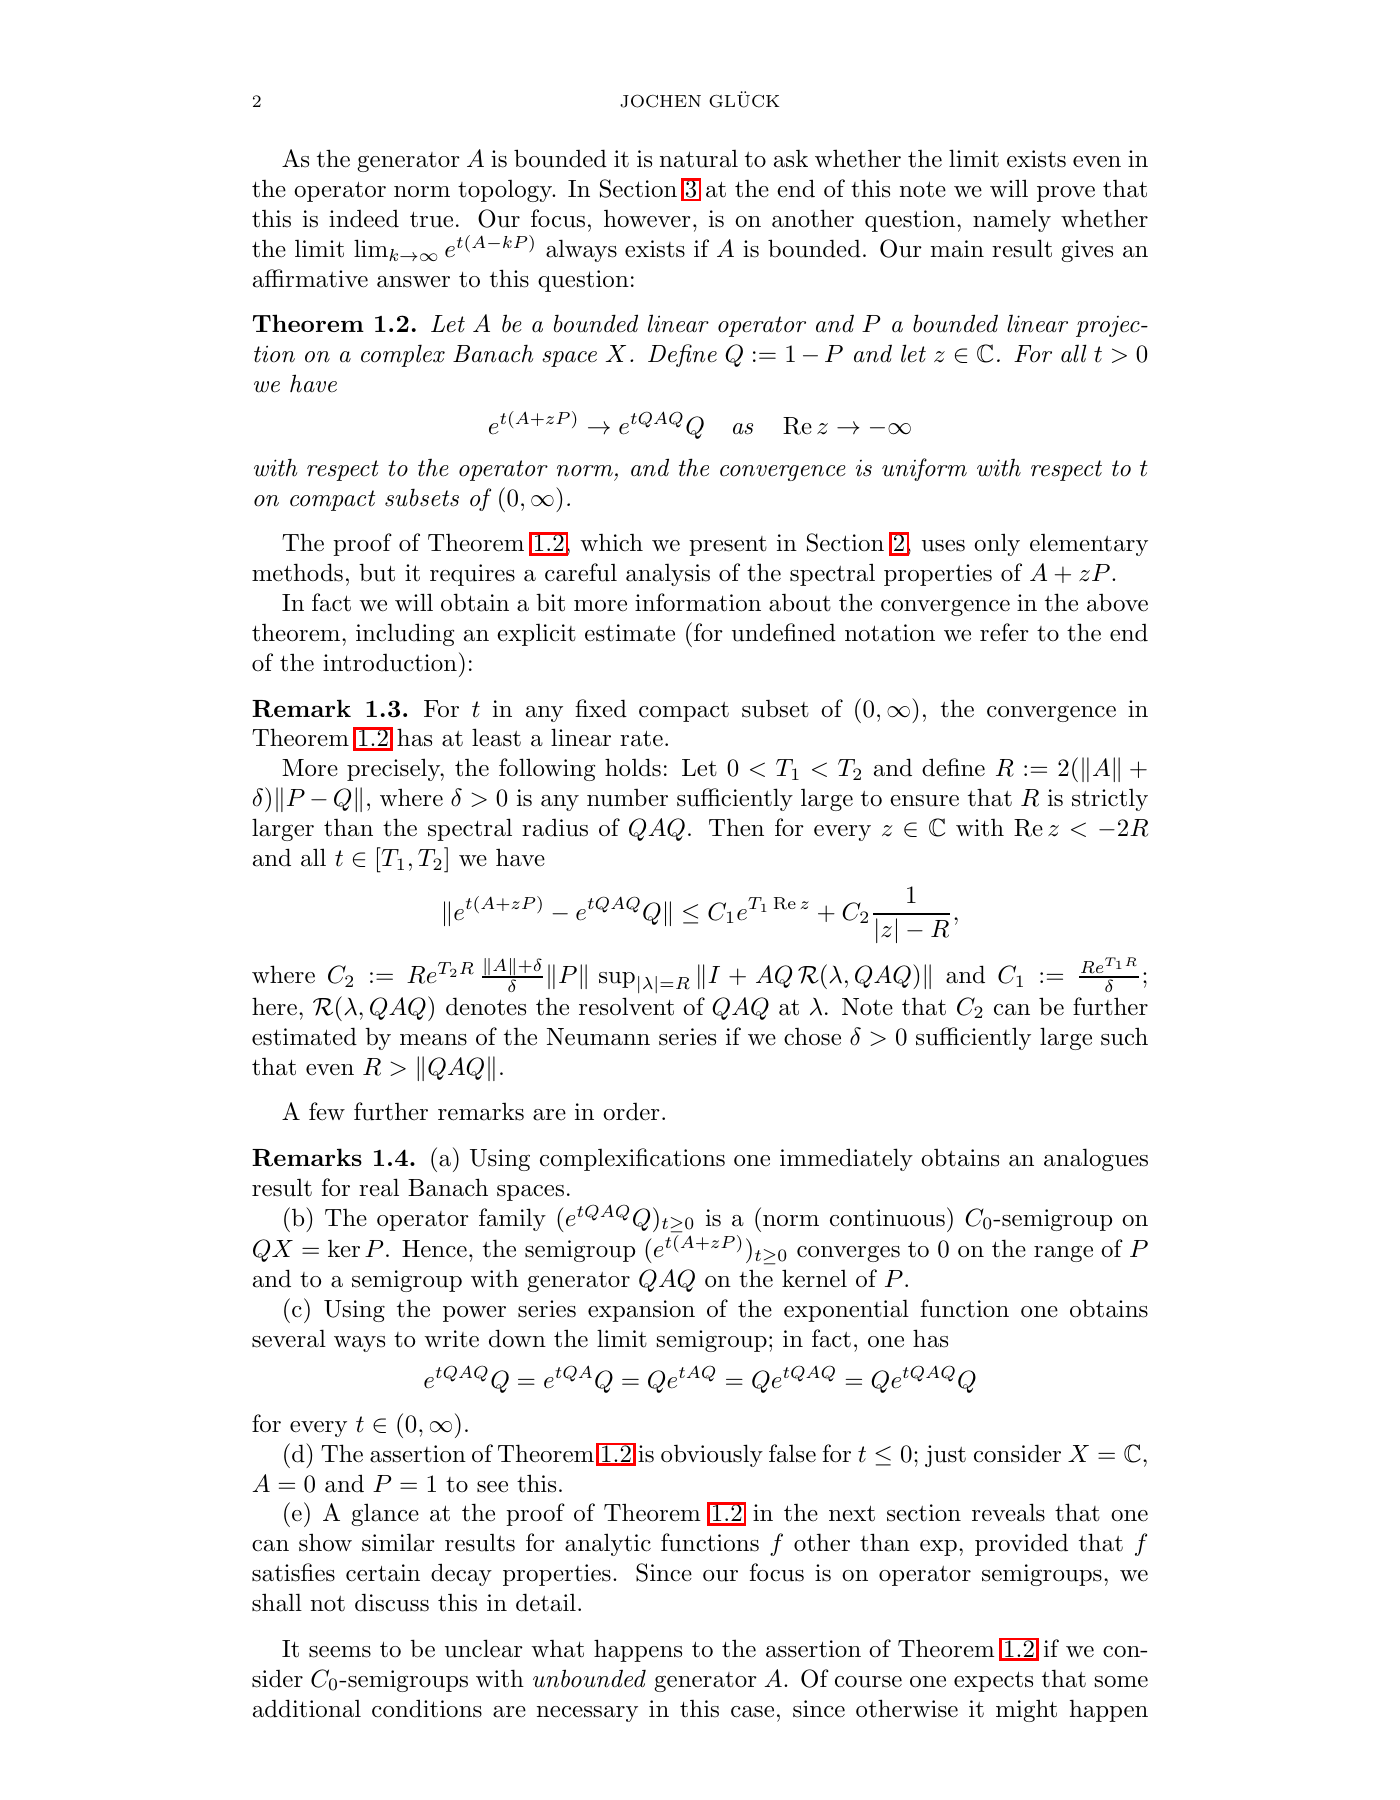
\includegraphics[width=0.92\textwidth,height=0.79\textheight,keepaspectratio]{figures/open_problem_crop_page2.png}
\caption{Source PDF page 2: Theorem~1.2, its operator-norm assertion, and the
beginning of the unbounded-generator question.}
\end{figure}
\clearpage

\begin{figure}[ht]
\centering
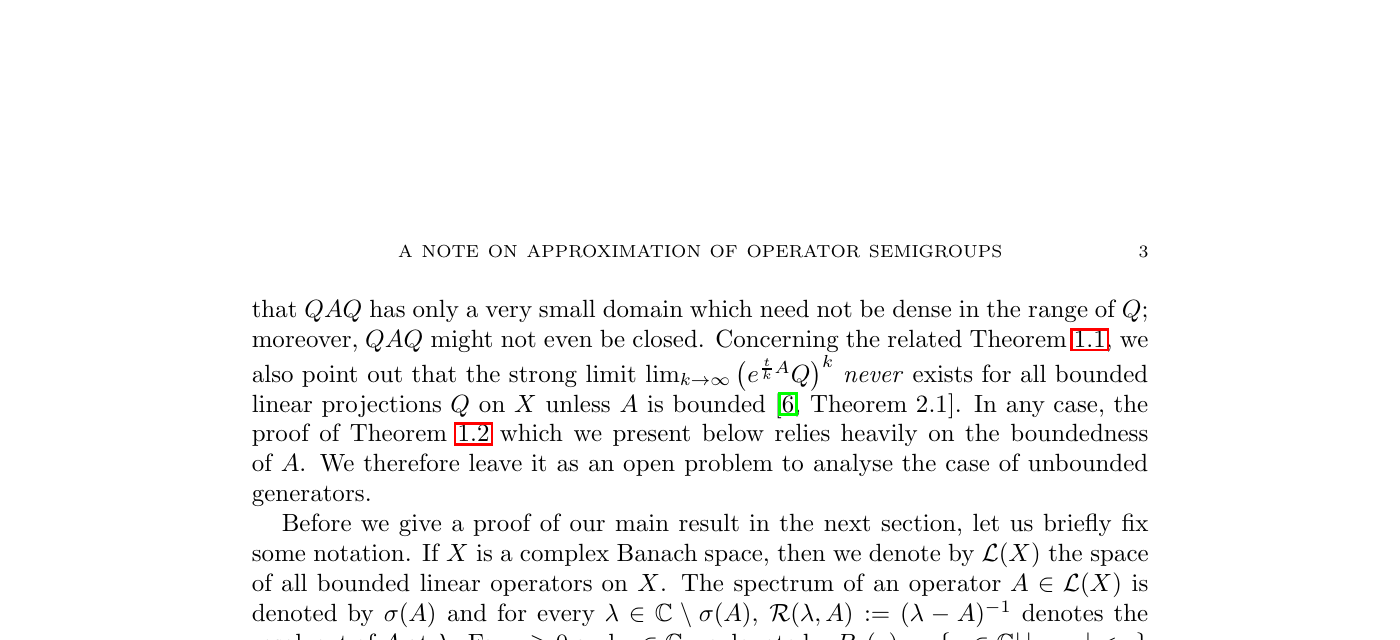
\includegraphics[width=0.96\textwidth]{figures/open_problem_crop_page3.png}
\caption{Source PDF page 3: continuation and explicit open-problem sentence.}
\end{figure}

\section{Proof intuition}

The bounded theorem controls all spectral modes using a constant depending on
$\opnorm{A}$. An unbounded generator has no such global frequency ceiling.
We exploit this with a direct sum of planar rotations of frequencies
$1,2,3,\ldots$ and damp the first coordinate at rate $k$.

For each fixed rotation block, letting $k\to\infty$ suppresses the first
coordinate and leaves the second coordinate fixed. Uniform contractivity then
gives strong convergence on the Hilbert direct sum. Operator norm can choose a
different block for each $k$: at frequencies $n\gg k$, fast rotation averages
the damping across both coordinates, so even the nominally undamped second
coordinate has size about $e^{-kt/2}$. The proposed limit $Q$ leaves that
coordinate unchanged. Their distance is therefore almost one.

\section{Construction and theorem}

Let
\[
 \Hh=\ell^2(\mathbb N;\mathbb C^2),\qquad
 J=\begin{pmatrix}0&-1\\1&0\end{pmatrix},
\]
and define
\[
 \D(A)=\left\{x=(x_n):\sum_{n\ge1}n^2\opnorm{x_n}^2<\infty\right\},
 \qquad (Ax)_n=nJx_n.
\]
Thus $A$ is an unbounded skew-adjoint operator and
$(e^{tA}x)_n=e^{tnJ}x_n$ is a unitary $C_0$-group. Define the orthogonal
projections, blockwise, by
\[
 P(a,b)=(a,0),\qquad Q(a,b)=(0,b).
\]

\begin{theorem}\label{thm:main}
For every $k>0$, $A-kP$ generates a contraction semigroup on $\Hh$. For every
$t>0$ and $x\in\Hh$,
\[
                   e^{t(A-kP)}x\longrightarrow Qx
                   \qquad(k\to\infty).
\]
However, for every fixed $t>0$,
\begin{equation}\label{eq:lower}
 \opnorm{e^{t(A-kP)}-Q}\ge 1-e^{-kt/2},
 \qquad
 \liminf_{k\to\infty}\opnorm{e^{t(A-kP)}-Q}\ge1.
\end{equation}
Consequently $e^{t(A-kP)}$ has no operator-norm limit as $k\to\infty$.
Moreover, $QAQ$ is zero on a dense domain in $Q\Hh$ and its closure is the
zero generator, so $Q=e^{t\overline{QAQ}}Q$ is precisely the natural compressed
semigroup predicted by Theorem~1.2.
\end{theorem}

\begin{proof}
Both $P$ and $Q$ preserve $\D(A)$. If $x\in\D(A)\cap Q\Hh$, then each
$x_n=(0,b_n)$ and $QnJx_n=0$. Hence $QAQ=0$ on the dense subspace
$\D(A)\cap Q\Hh$ of $Q\Hh$, and its closure is zero on all of $Q\Hh$.

The $n$th block of $A-kP$ is
\[
                   M_{n,k}=\begin{pmatrix}-k&-n\\n&0\end{pmatrix}.
\]
If $v'(t)=M_{n,k}v(t)$, then
\[
       \frac{d}{dt}\opnorm{v(t)}^2
          =2\operatorname{Re}\langle M_{n,k}v(t),v(t)\rangle
          =-2k|v_1(t)|^2\le0.
\]
Thus every block exponential is a contraction. Their Hilbert direct sum is a
strongly continuous contraction semigroup, and its generator is $A-kP$.

We first prove strong convergence. Fix $n$. Once $k>2n$, put
\[
 \delta=\sqrt{k^2/4-n^2},\qquad
 \lambda_\pm=-k/2\pm\delta.
\]
The exact two-by-two exponential is
\begin{equation}\label{eq:overdamped}
 e^{tM_{n,k}}
 =\frac{e^{t\lambda_+}+e^{t\lambda_-}}2 I
 +\frac{e^{t\lambda_+}-e^{t\lambda_-}}{2\delta}
       \left(M_{n,k}+\frac{k}{2}I\right).
\end{equation}
As $k\to\infty$, $\lambda_+\to0$, $\lambda_-\to-\infty$,
$k/(2\delta)\to1$, and $n/\delta\to0$. Formula
\eqref{eq:overdamped} therefore gives
\[
             e^{tM_{n,k}}\longrightarrow
             Q_2:=\begin{pmatrix}0&0\\0&1\end{pmatrix}
\]
for every fixed $n$ and $t>0$. Hence convergence holds on finitely supported
vectors. Since both $e^{t(A-kP)}$ and $Q$ are contractions, a finite-support
approximation gives convergence for every $x\in\Hh$.

It remains to show that this convergence is not uniform on the unit ball.
Fix $k,t>0$, and let $n>k/2$. With
$\omega=\sqrt{n^2-k^2/4}$, the underdamped formula gives
\begin{equation}\label{eq:underdamped}
 e^{tM_{n,k}}e_2=e^{-kt/2}
 \begin{pmatrix}
 -\dfrac{n}{\omega}\sin(\omega t)\\[4pt]
 \cos(\omega t)+\dfrac{k}{2\omega}\sin(\omega t)
 \end{pmatrix}.
\end{equation}
As $n\to\infty$, $n/\omega\to1$ and $k/(2\omega)\to0$, so uniformly in the
oscillating phase,
\[
                    \opnorm{e^{tM_{n,k}}e_2}\longrightarrow e^{-kt/2}.
\]
Let $f_n\in\Hh$ be the unit vector equal to $e_2$ in block $n$ and zero
elsewhere. Since $Qf_n=f_n$, the reverse triangle inequality yields
\[
 \opnorm{e^{t(A-kP)}-Q}
 \ge \opnorm{e^{tM_{n,k}}e_2-e_2}
 \ge 1-\opnorm{e^{tM_{n,k}}e_2}.
\]
Letting $n\to\infty$ proves the first inequality in \eqref{eq:lower}, and then
$k\to\infty$ proves the second. Any operator-norm limit would have to equal
the already established strong limit $Q$, so no operator-norm limit exists.
\end{proof}

\section{Verification, novelty, and scope}

\paragraph{Verification.}
The proof uses exact matrix exponentials. The included regression script
checks fixed-mode convergence, high-frequency asymptotics, the lower bound,
and contractivity over several parameter ranges. It is not part of the proof.

\paragraph{Bounded novelty search.}
The four run indexes were searched for arXiv:1511.02329, absorption semigroups,
unbounded generators, projection damping, rotation blocks, and operator-norm
convergence. Exact-title, exact-phrase, author/id, formula, quantum-Zeno, and
close-variant arXiv/web searches through 27 August 2026 found generic references
to the source but no exact answer. OpenAlex and Semantic Scholar citation
metadata for the source DOI returned no indexed citing works. Novelty is
plausible, not certified.

\paragraph{Scope and review.}
This completely disproves the unconditional operator-norm extension of
Theorem~1.2 to arbitrary unbounded generators. It does not classify useful
additional assumptions (analyticity, compact resolvent control, invariant
domains, or spectral cutoffs) that restore convergence, so the source's broad
request to analyse the unbounded case remains open beyond this negative
boundary result. Human review should check formulas
\eqref{eq:overdamped}--\eqref{eq:underdamped} and the finite-support density
argument.

\begingroup
\sloppy
\raggedright
\begin{thebibliography}{9}
\bibitem{Glueck}
J.~Gl\"uck,
\emph{A note on approximation of operator semigroups},
Arch. Math. (Basel) \textbf{106} (2016), 265--273;
\href{https://arxiv.org/abs/1511.02329}{arXiv:1511.02329}.
\end{thebibliography}
\endgroup
\end{document}
